In this chapter the planning and work-flow regarding Sprint 4 will be described. 
Everything from setting our goals to implementation and testing. At the end the team will evaluate the whole sprint and try on answer the following questions: What went well? What could be improved? 
\section{Sprint planning}

The customer was very satisfied with the demonstration video for sprint 3. The team planned how to take the project further. At this point it was possible to send control signals to multiple clients, and then detect the devices that lit up. It was decided that the plan for this sprint was to combine those two, and try to create an image, more specific a traffic light. This meant that after detection the signal should make the first client light up red, and make the second one light up yellow, and then make the last one light up green. Since the main goal was to make the mobile screens create an image, the order of the different colors was be imporant. The team had to plan for making specific devices to light up specific colors at spesific positions. A traffic light was a good start for focusing on this part of the assignment, and the customer agreed. For sprint 4, the plan was to first map all available devices to grid, and then link the devices location with their ids, and then make the clients create a traffic light.  


In sprint 4 the team also planned to work more on the report. The plan was to finish sprint 3, since that sprint finished the week before. It was also wanted to start working on sprint 4. Since it was implemented detection of devices, and it was planned to link their location to their ids, it was decided that it was imporant to add more information about the software architecture as well. The team where also getting a better understanding of what the end product would look like, therefore it was planned to start working a little bit on the evaluation as well. The supervisor also came up with some suggestions for small improvements on the report, which the team planned to follow up. Also it was decided to make to the user stories more consistent. It was also planned to separate the implementation stories from the documentation, and the project management stories.


All implementation related stories for sprint 4 are presented in table \ref{tab:sprint4stories}.
%\caption{User stories selected for Sprint 4.}
  \label{tab:sprint4stories}
 \def\arraystretch{1.25}
 
\begin{longtable}{ccXcc}

\toprule[0.5mm]
\multirow{2}{*}{\textbf{ID}} &
\multirow{2}{*}{\textbf{Ref.}} & \multirow{2}{*}{\textbf{Description}} & \multicolumn{2}{c}{\textbf{Hours}} \\
 					& & & \textbf{Est.} & \textbf{Sp.} \\
%\textbf{ID} 	& \textbf{Description} 	& \textbf{Est.} & \textbf{Sp.} \\
\midrule
\textbf{I4.1} 	& 	& {\bf As a server I need to link the devices' location with their ids.}	 &  52	& \textbf{48} \\

\textbf{I4.2} 	& 	& {\bf As a server I need to identifiy multiple clients from light.}		 &  19	& \textbf{18} \\

\textbf{I4.3} 	& 	& {\bf As a server I need to map all available devices to grid.} 			 & 22 & \textbf{18} \\	

\textbf{I4.4} 	& 	& {\bf As a server I need to play the whole media to the grid.} 			 & 37 & \textbf{34} \\
	
\midrule
		
				&& \textbf{SUM:}		&		130	& \textbf{136}
 \\																			
\bottomrule[0.5mm]
\end{longtable}


All the documentation related stories for sprint 4 are presented in table \ref{tab:sprint4Documentationstories}.
%\caption{User stories selected for Sprint 2.}
\def\arraystretch{1.25}
 
\begin{longtable}{ccXcc}
\label{tab:sprint2Documentationstories}\\[-6mm]
\caption{Documentation stories selected for sprint 2}\\[-4mm]
\toprule[0.5mm]
\multirow{2}{*}{\textbf{ID}} &
\multirow{2}{*}{\textbf{Ref.}} & \multirow{2}{*}{\textbf{Description}} & \multicolumn{2}{c}{\textbf{Hours}} \\
 					& & & \textbf{Est.} & \textbf{Sp.} \\
%\textbf{ID} 	& \textbf{Description} 	& \textbf{Est.} & \textbf{Sp.} \\
\midrule


\textbf{D2.1} 	& 
	\refwbs{wbs_documentation}{WBS 8.2}	& {\bf As a student I need to finish the pre-study chapter.} 									& 	12	& \textbf{ 16} \\

\textbf{D2.2} 	& 
	\refwbs{wbs_documentation}{WBS 8.2}	& {\bf As a student I need to finish the planning chapter.} 									& 	10	& \textbf{ 14} \\

\textbf{D2.3} 	&
	\refwbs{wbs_documentation}{WBS 8.2} 	& {\bf As a student I need to finish requirements chapter.} 									& 	30	& \textbf{ 26} \\

\textbf{D2.4} 	& 
	\refwbs{wbs_documentation}{WBS 8.2}  & {\bf As a student I need to finish the architecture chapter.} 								& 	24	& \textbf{ 12} \\

\textbf{D2.5} 	& 
	\refwbs{wbs_documentation}{WBS 8.2}	& {\bf As a student I need to finish sprint 1 chapter.} 										& 	12	& \textbf{ 16} \\

\textbf{D2.6} 	& 
	\refwbs{wbs_documentation}{WBS 8.2}	& {\bf As a student I need to work on the  sprint 2 chapter.} 									& 	16	& \textbf{ 18} \\
%ASK group about this:
%\textbf{360} 	& \refreq{}
%	& {\bf As a student I need to start on the architechture chapter.} 								& 	?	& \textbf{ ?} \\	

								
\hline
				&& \textbf{SUM:}		&		104	& \textbf{102}
 \\																			
\bottomrule[0.5mm]
\end{longtable}

All the project management related stories for sprint 4 are presented in table \ref{tab:sprint4storiesProcess}.
%\caption{User stories selected for Sprint 1.}
\label{tab:sprint1storiesProcess}
\def\arraystretch{1.25}
 
\begin{longtable}{ccXcc}

\toprule[0.5mm]
\multirow{2}{*}{\textbf{ID}} &
\multirow{2}{*}{\textbf{Ref.}} & \multirow{2}{*}{\textbf{Description}} & \multicolumn{2}{c}{\textbf{Hours}} \\
 					& & & \textbf{Est.} & \textbf{Sp.} \\
%\textbf{ID} 	& \textbf{Description} 									& \textbf{Est.} & \textbf{Sp.} \\
\midrule

% === Process ==========================
\textbf{326} 	& 
	& {\bf  As a student I have to track effort time} 	& 		16	& \textbf{16} \\
\textbf{345} 	& 
	& {\bf As a student I have attend the weekly meetings with the customer} 	
	& 	22	
	& \textbf{?} \\
		&& Preparation for demonstration	& 2 & ? \\
		&& Demonstration	& 6 & ? \\
		&& Writing minutes 	&  6 & ? \\	
		&& Customer meeting	&  6 & ? \\
		&& Writting minutes	&  2 & ? \\
		
\textbf{327} 	& 
	& {\bf As a student I have to attend the weekly meetings with the supervisor} 	
	& 	12	
	& \textbf{?} \\
		&& Meeting in week I	& 4 & ? \\
		&& Meeting in week II	& 4 & ? \\
		&& Writing minutes from week I 	&  2 & ? \\
		&& Writing minutes from week II	&  2 & ? \\	

\textbf{344} 	&& {\bf As a student I need to attend the team building.} 	& 		7	& \textbf{9} \\
		

\textbf{321} 	&& {\bf As a student I need to participate to lectures about team dynamics. } 	& 		32	& \textbf{25} \\
				&& Course of group dynamics Thu.	&  &  \\
				&& Summary of course and exchange learned.	&  &  \\				
				
\hline
				&& \textbf{SUM:}		&		164	& \textbf{?}
 \\																			
\bottomrule[0.5mm]
\end{longtable}


% hous all in total: Estimated: 130 + 65 + 42 = 237  Spent: 136+ 36+35= 207

\subsection{Duration}
This sprint is 2 weeks long. From 14th of October 2013 to 27th of October 2013. We agreed
on the date of presentation and showing the running demo – on Thursday 25th of October 2013.
Estimated velocity is 240 hours since we agreed on 30 working hours per person per week.

\section{Preliminary studies}
% TODO
\section{Sprint goal}

The goal for sprint 4 is to link the devices location with their ids, and then make the clients create a traffic light together. 
\begin{figure}[H]
	\centering
		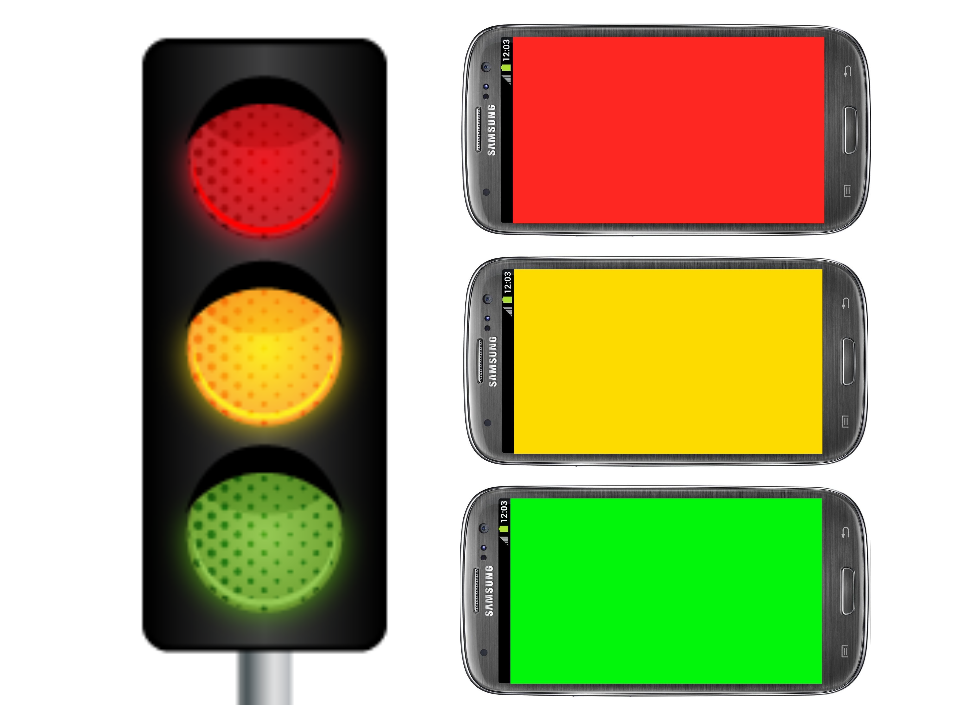
\includegraphics[width=10cm]{sprint4/trafficlight.png}
	\caption{Traffic Light.}
	\label{fig:trafficlight }
\end{figure}

\section{System Burndown}
\begin{figure}[H]
	\centering
		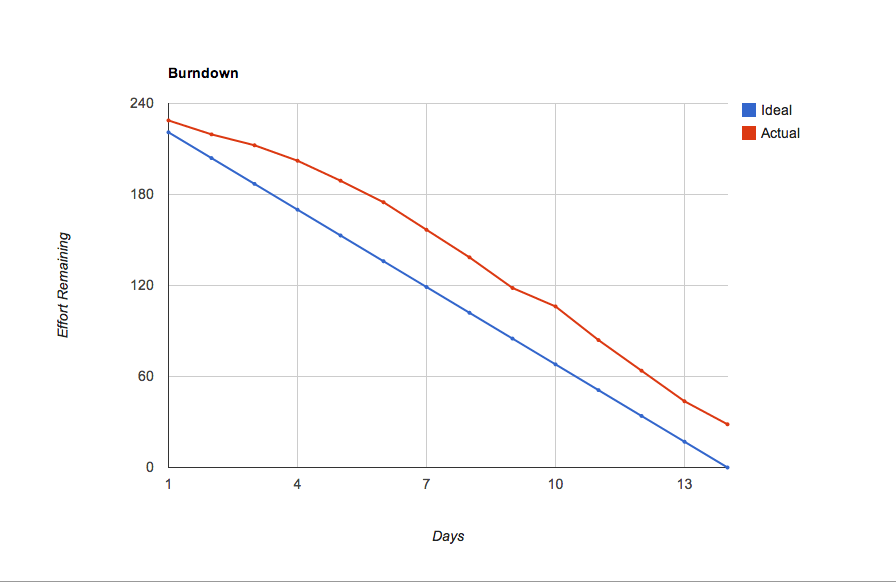
\includegraphics[width=18cm]{sprint4/BurndownSprint4.png}
	\caption{Burn down chart.}
	\label{fig:Burn4 }
\end{figure}
\section{Architecture}
\section{Implementation}
\section{Testing}
\section{Occurring risks}
\section{Customer feedback}
\section{Retrospective}
This section reflects on the past sprint. In order to learn from the mistakes done and thus to improve the workflow it is necessary to answer two essential questions: "What went well" and "What could be improved".

\subsection{What went well}
\subsection{What could be improved}
